\documentclass{article}
\usepackage[utf8]{inputenc}
\usepackage{float}
\usepackage{amsmath,amssymb,amsthm,graphicx}
\usepackage{subcaption}
\usepackage{tikz}
\usepackage{tikz-network}

\setlength{\oddsidemargin}{0.25 in}
\setlength{\evensidemargin}{-0.25 in}
\setlength{\topmargin}{-0.6 in}
\setlength{\textwidth}{6.5 in}
\setlength{\textheight}{8.5 in}
\setlength{\headsep}{0.75 in}
\setlength{\parindent}{0 in}
\setlength{\parskip}{0.1 in}

\newtheorem{theorem}{Theorem}
\newtheorem{corollary}{Corollary}
\newtheorem{proposition}{Proposition}
\newtheorem*{remark}{Remark}
\theoremstyle{definition}
\newtheorem{example}{Example}
\newtheorem{definition}{Definition}

\newcommand{\lecture}[4]{
   \pagestyle{myheadings}
   \thispagestyle{plain}
   \newpage
%   \setcounter{lecnum}{#1}
   \setcounter{page}{1}
   \noindent
   \begin{center}
   \framebox{
      \vbox{\vspace{2mm}
    \hbox to 6.58in { {\bf CSC~565: Graph Theory
                        \hfill North Carolina State University} }
    \hbox to 6.58in { {\bf Fall 2019
                        \hfill Computer Science} }
       \vspace{4mm}
       \hbox to 6.28in { {\Large \hfill Lecture #1: #2  \hfill} }
       \vspace{2mm}
       \hbox to 6.28in { {\it Lecturer: {\it Don Sheehy {\tt <drsheehy@ncsu.edu>}} \hfill Scribe: #4} }
      \vspace{2mm}}
   }
   \end{center}
   \markboth{Lecture #1: #2}{Lecture #1: #2}
   \vspace*{4mm}
}


\begin{document}
%FILL IN THE RIGHT INFO.
%\lecture{**LECTURE-NUMBER**}{**DATE**}{**LECTURER**}{**SCRIBE**}
\lecture{29}{Dec 4, 2019}{Hongyi Fan, Guangyu Yu Scribe}
%\footnotetext{These notes are partially based on those of Nigel Mansell.}

% **** YOUR NOTES GO HERE:

% Some general latex examples and examples making use of the
% macros follow.  
%**** IN GENERAL, BE BRIEF AND COMPLETE. 



\section{P and NP problem} 
\begin{definition}
decision problem with polynomial solutions is called \textbf{P problem}
\end{definition}


If A is a decision problem, $V_{A}$ is called \textbf{verifier} if
\[
A = \{a\; | <a, b> \in V_A  \; \text{for some b} \}
\]
\begin{definition}
decision problem with polynomial verifiers is called \textbf{NP problem}
\end{definition}

\section{Polynomial-time reduction} 
Consider A and B are decision problems, and f : Instance of A $\to$  Instance of B,\\
\\
Requirement 1:
\[
a \in A \; \text{iff} \; f(a) \in B
\]
Requirement 2:
\[
\textmd{f runs in polynomial time}
\]

Denotation:
\[
A \leq_{p} B
\]
Example:
\begin{figure}[h!]
		\begin{center}
			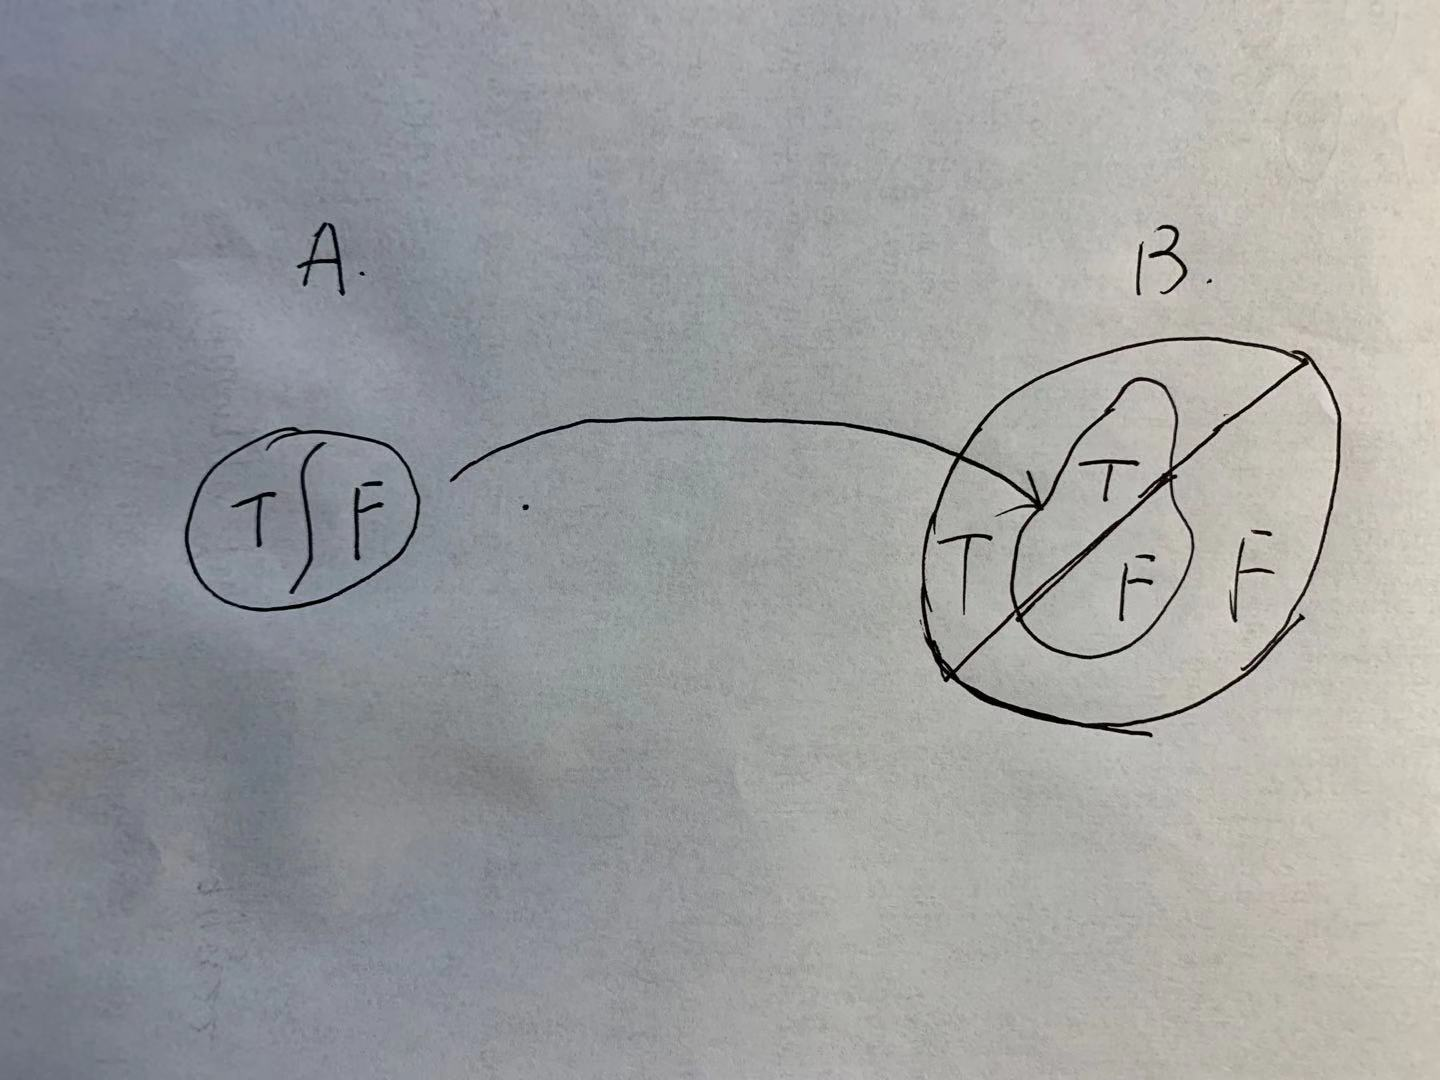
\includegraphics[scale=0.10]{images/fig4}
		\end{center}
		\caption{Polynomial time reduction}
	\end{figure}

\section{NP-complete problem} 
\begin{definition}
If A is a decision problem and A $\in$ NP, such that
\[
\forall B \in \text{NP}, \;  B \leq_{p} A
\]
then A is called \textbf{NP-complete problem}
\end{definition}

\subsection{SAT problem} 

\textbf{SAT problem:} determining if there exists an interpretation that satisfies a given boolean expression.

Example:
\[
(x_{1} \lor \bar x_{2} \lor x_{3} \lor x_{4})\land (x_{4} \lor x_{2} \lor \bar x_{5})
\]
\begin{theorem}
SAT problem is NP-complete
\end{theorem}

\subsection{VC(vetex cover) problem} 
\begin{definition}
A \textbf{vetex cover(VC)} is a subset $V^{'}$ $\in$ $V$, such that
\[
\forall e \in E, \; e \cap V^{'} = \oslash
\]
\end{definition}
\textbf{VC problem:} given a Graph $G$ and size $k$, does $G$ have a VC of size $k$?

\subsection{3SAT  $\leq_{p}$ VC } 

  Transformation rules from boolean expression to graph G:\\
\[
\forall \; \text{variable} \; x \to x, \bar x \in V, (x, \bar x) \in E 
\]
\[
\forall \; \text{clause} \; (a \lor b \lor c) \to a, b, c \in V, (a,b), (a,c), (b,c) \in E
\]

  Consider 3SAT expression consists n variables and m clauses. 
\begin{itemize}
\item[-] For every triangle generated by the clauses, we need at least 2 vertices in our VC otherwise we can't cover 3 edges in this triangle, so we need at least $2m$ vertices in our VC.
\item[-] For every edge generated by the variables, we need at least 1 vertices in our VC to cover this edge, so we need at least $n$ vertices in our VC. 
\end{itemize}
In summary, the size $k$ of VC is at least $2m + n$, that is
\[
\text{If Exp} \in \text{3SAT, then} (G, 2m+n) \in VC 
\]

\textbf{So, VC problem is NP-complete}

\subsection{IS(independent set) problem} 
\begin{definition}
A \textbf{independent set(IS)} is a set of $v$ such that no two of which are adjacent.
\end{definition}
\textbf{IS problem:} given a Graph $G$ and size $k$, does $G$ have a IS of size $k$?\\

Relation between VC and IS: 
\[
V^{'} \in V \; \text{is a VC iff} \; V\setminus V^{'} \text{is an IS.}
\]
in another word,
\[
(G, k) \in \text{VC} \; \text{iff} \; (G, n-k) \in \text{IS}
\]

\textbf{So, IS problem is NP-complete}

\subsection{Clique problem} 
\begin{definition}
A \textbf{clique} is a subset of $V$ such that every two distinct vertices in the clique are adjacent
\end{definition}
\textbf{Clique problem:} given a Graph $G$ and number $k$, does $K_{k} \in G$?\\

Relation between IS and clique:
\[
(G, k) \in \text{IS iff} \; (\bar G, k) \in \text{clique}
\]

\textbf{So, clique problem is NP-complete}

\subsection{Subgraph Isomophism(SubGI) problem} 
\textbf{SubGI problem:} given a Graph $G$ and $H$, does $G$ have a subgraph isomorphic to $k$?\\

Relation between clique and SubGI:
\[
(G, k) \in \text{clique iff} \; (G, K_{k}) \in \text{SubGI}
\]

\textbf{So, SubGI problem is NP-complete}

\end{document}